\section{Financing}
\subsection{Pricing and cost}\label{pricing}
\begin{wrapfigure}{R}{0.5\textwidth}
  \centering
   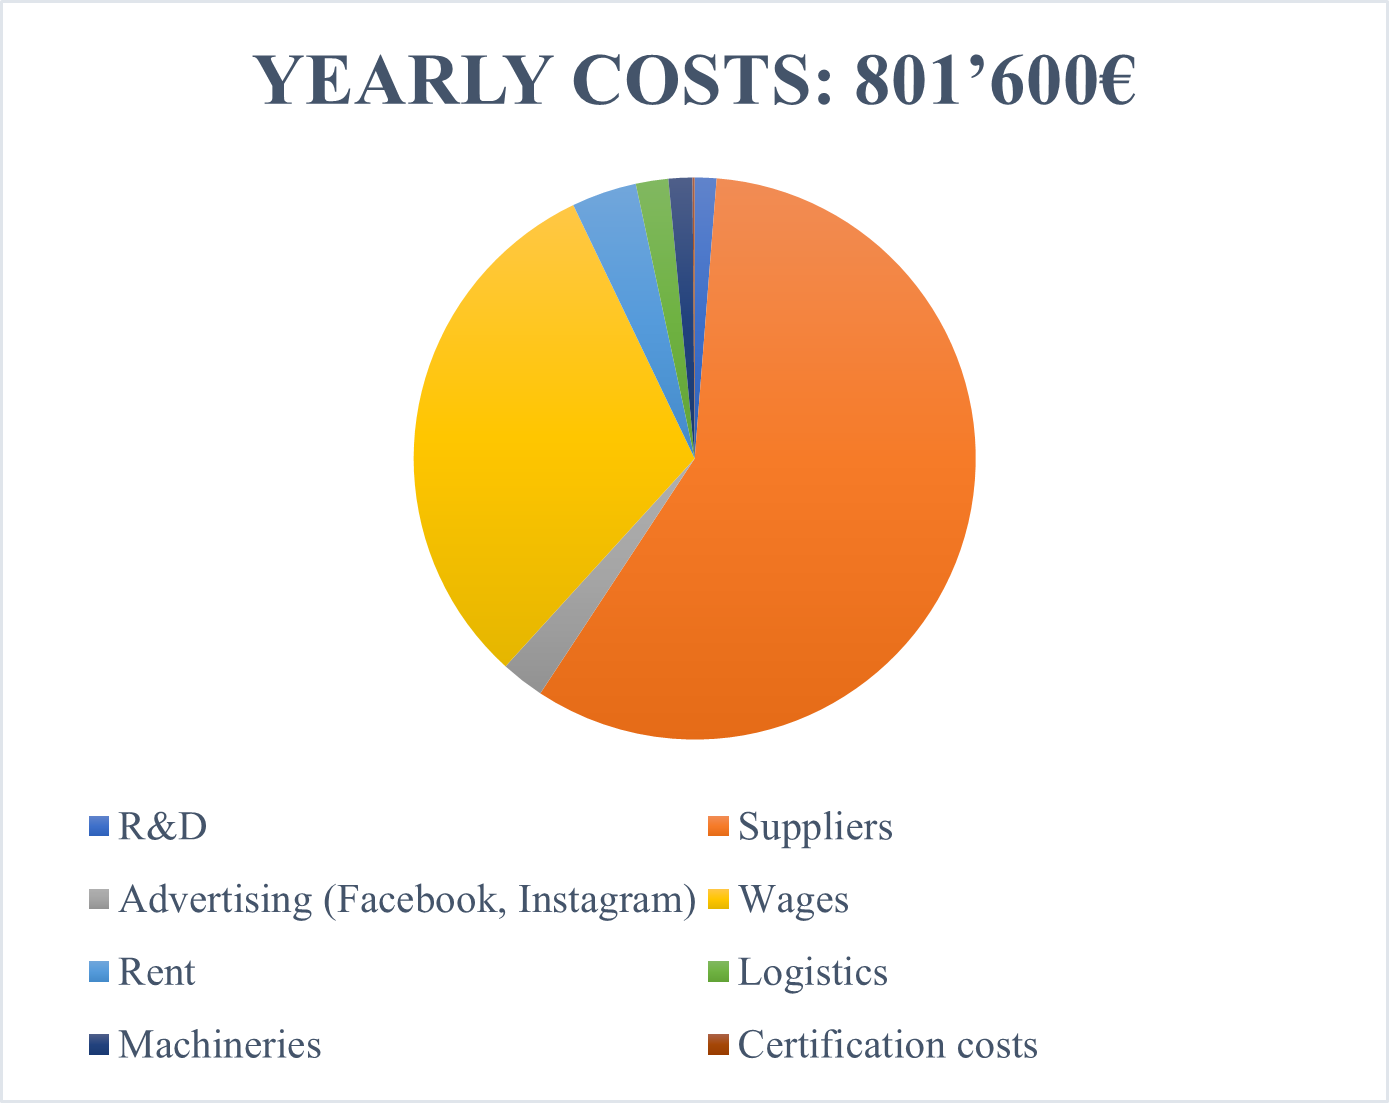
\includegraphics[width=0.48\textwidth]{images/costi-diagramma-torta.png}
  \caption{YEARLY COSTS Diagram}
\end{wrapfigure}
YEARLY COSTS: 801’600€\\
\begin{itemize}
\item \textbf{R\&D}: 10’000€
\item \textbf{Suppliers}: 465’000€
\item \textbf{Advertising} (social media): 20’000€
\item \textbf{Wages}: 249’600€
\item \textbf{Rent}: 30’000€
\item \textbf{Logistics}: 15’000€
\item \textbf{Machinery}: 11’000€
\item \textbf{Certification costs}: 1’000€
\end{itemize}
(of which Fixed Costs: 336’000€)
\begin{table}[H]
\centering
\caption{prices of our products}
\begin{tabular}{GGccccm{0.1\textwidth}}
\toprule
& Components & 1st Year Scale & Cost & Price & Margin\\
\hline
OPTION 1 (food container)& Case double layered + Cap + Electronic Parts & 3000 units & 30€ & 40€ & 10€\\
\hline
OPTION 2 (water bottle)& Case double layered + Cap & 3000 units & 13€ & 25€ & 12€\\
\hline
OPTION 1+2 (food + water bottle)& Cases double layered + Cap + Electronic Parts & 15000 units &45€ & 55€ & 10€\\
\bottomrule
\end{tabular}
\end{table}

\newpage
\subsection{Costs of the products}
\subsubsection*{COSTS OF OPTION 1 “FOOD CONTAINER”: 30€}
     \begin{table}[h!]
     \begin{center}
     \begin{tabular}{  p{0.45\textwidth} c}
     
      \begin{itemize}[topsep=0pt]
      \item[\textbf{11€}] Electronic parts (APPENDIX A)
      \item[\textbf{7€}] Double layered case
      \item[\textbf{0.5€}] Cap
      \item[\textbf{0.5€}] Package
      \item[\textbf{11€}] Fixed Costs 
      \end{itemize}
	  &
	  \raisebox{-\totalheight}{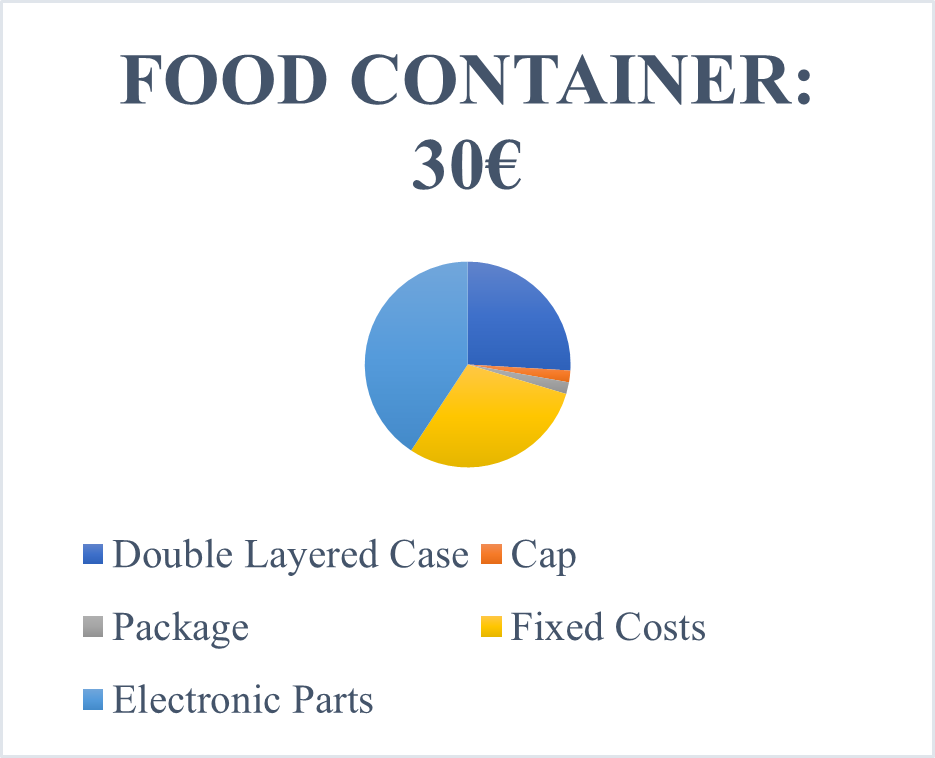
\includegraphics[width=0.48\textwidth]{images/food_container.png}}
      \\
      \end{tabular}
      \label{tbl:myLboro}
      \end{center}
      \end{table}
\subsubsection*{COST OF OPTION 2 “WATER BOTTLE”: 13€}
     \begin{table}[h!]
     \begin{center}
     \begin{tabular}{  p{0.45\textwidth} c}

      \begin{itemize}[topsep=0pt]
      \item[\textbf{6€}] Double layered case
      \item[\textbf{0.5€}] Cap
      \item[\textbf{0.5€}] Package
      \item[\textbf{6€}] Fixed Costs 
      \end{itemize}
	  &
	  \raisebox{-\totalheight}{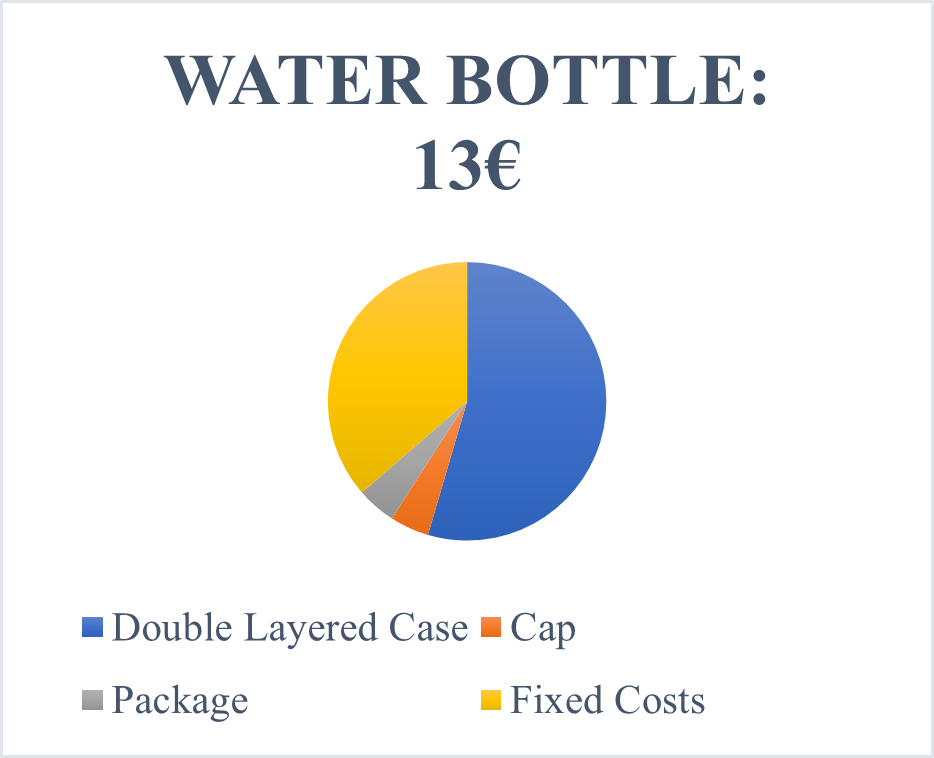
\includegraphics[width=0.48\textwidth]{images/water_bottle.png}}
      \\
      \end{tabular}
      \label{tbl:myLboro}
      \end{center}
      \end{table}
      \newpage
\subsubsection*{COST OF OPTION 1+2 “WATER+FOOD CONTAINER”: 45€}
     \begin{table}[h!]
     \begin{center}
     \begin{tabular}{  p{0.45\textwidth} c}

      \begin{itemize}[topsep=0pt]
      \item[\textbf{11€}] Electronic parts (APPENDIX A)
      \item[\textbf{13€}] Double layered case
      \item[\textbf{1€}] Cap
      \item[\textbf{1€}] Package
      \item[\textbf{19€}] Fixed Costs 
      \end{itemize}
	  &
	  \raisebox{-\totalheight}{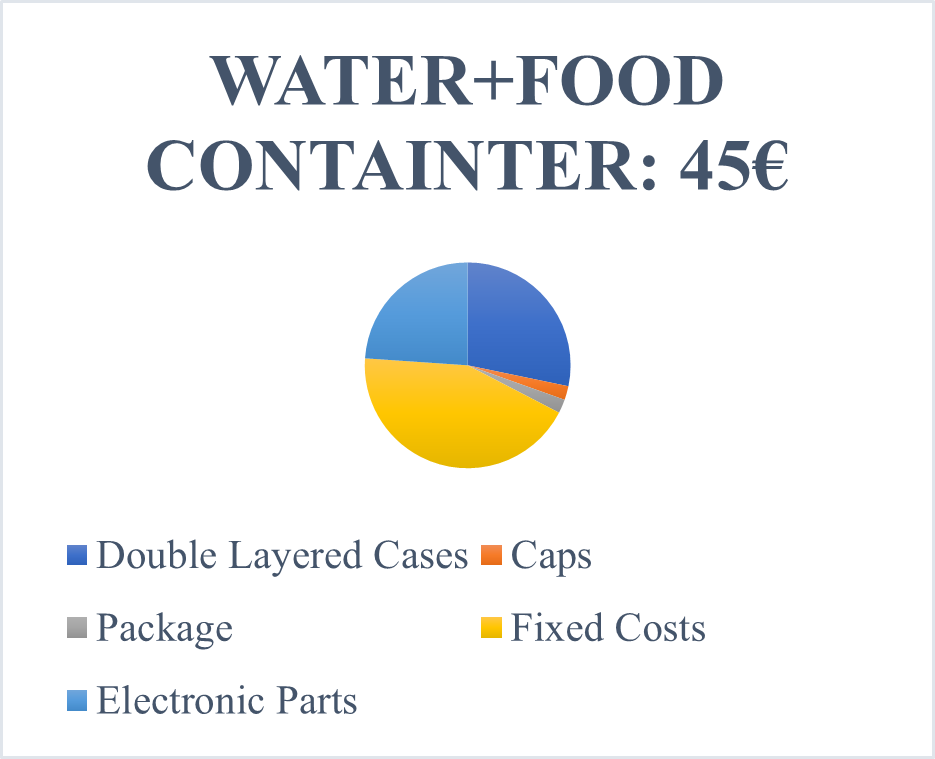
\includegraphics[width=0.48\textwidth]{images/water+food.png}}
      \\
      \end{tabular}
      \label{tbl:myLboro}
      \end{center}
      \end{table}
\FloatBarrier
\subsection{Fixed Costs}
\subsubsection*{WAGES: 249’600€}
\textbf{WORKERS}: 1700*12 *4PP =81’600€\\
\textbf{EMPLOYEES}: 2000*12 *2PP = 48’000€ (Accounting, Quality Check, Costumer Relationship)\\
\textbf{TEAM FOUNDERS}: 2000*12 *5pp =120’000€ (Management, R\&D, App development, HR)
\subsubsection*{RENT} 
\textbf{Facility Renting} 2’500€ per month
\subsubsection*{LOGISTICS}
About 15’000€ shipping prices with DHL according to yearly shipping volumes
\subsubsection*{MACHINERY} 
5’000€ personal computers for employees
3’000€ for manufacturing (soldering station, PCs, others)
\subsubsection*{CE CERTIFICATION}
1000€ per year [7]

\subsection{Our Pricing Strategy}
The pricing strategy is very simple. We compare our product to competitors' prices, then we introduce our prices according to what our product offers more with respect to competitors and how much our costumers are willing to pay for it.
\subsubsection*{Payment Options}
At BottAll Company, our payment policy is all inclusive because we are quite aware that different people prefer different payment options as it suits them. Here are the payment options that will be available at our retailers and on the website;\\
Payment by cash at retailers\\
Online payments:
\begin{itemize}
\item PayPal.
\item Apple Pay.
\item Amazon Pay.
\item Google Pay.
\item Payment via online bank transfer (VISA/Mastercard circuits)
\end{itemize}

\subsection{Financial Fundings}
\subsubsection*{Personal Investment}

Our company will start relying on our own investment. The founding team will gather an amount of 100'000€ based on our own savings and through the help of our families and friends. This money is intended to start the project, develop the design of the product and at least complete the prototyping period. 

\subsubsection*{Debt Capital} 

After the first period we are going to need a considerable amount of money in order to pay for the facility we are going to rent, for all the needed equipment inside the facility and also for the first orders to suppliers.\\
Our idea is to ask for a loan to the bank of 100'000€. This money will be enough for the facility and the equipment and also for a small number of components. In this way we can finally start the production.

\subsubsection*{Kickstarter}

As far as we start the production, we will launch a Kickstarter campaign in order to raise the money needed for continuing the manufacturing and to guarantee small time delivery to our customers. \\
Goal: the target of our company is to reach 50'000€ with a Kickstarter campaign selling our products with a remarkable discount to the future price. \\
Doing any purchase during the Kickstarter campaign, the costumer will be able to keep in touch with us through a newsletter and a dedicated “Facebook group” where everyone can express their opinions and suggestions. For everyone who bought the complete package (food + water) we will organize private zoom calls with them (once a month) where selected financier (via booking) can discuss directly with us for hints and explanations. A more detailed view of the Kickstarter campaign in Appendix A.

\subsubsection*{Equity based Crowdfunding} 

Last but not least, as soon as our company is well establish in the market we are going to sell a small share of the society, indicatively a 20\% share for 250'000€, in order to have liquidity to pay wages and suppliers for increasing our market and reach the expected production numbers set at the initial phase of the company. 



\subsection{Financial Projection}
\begin{figure}[H]
\centering
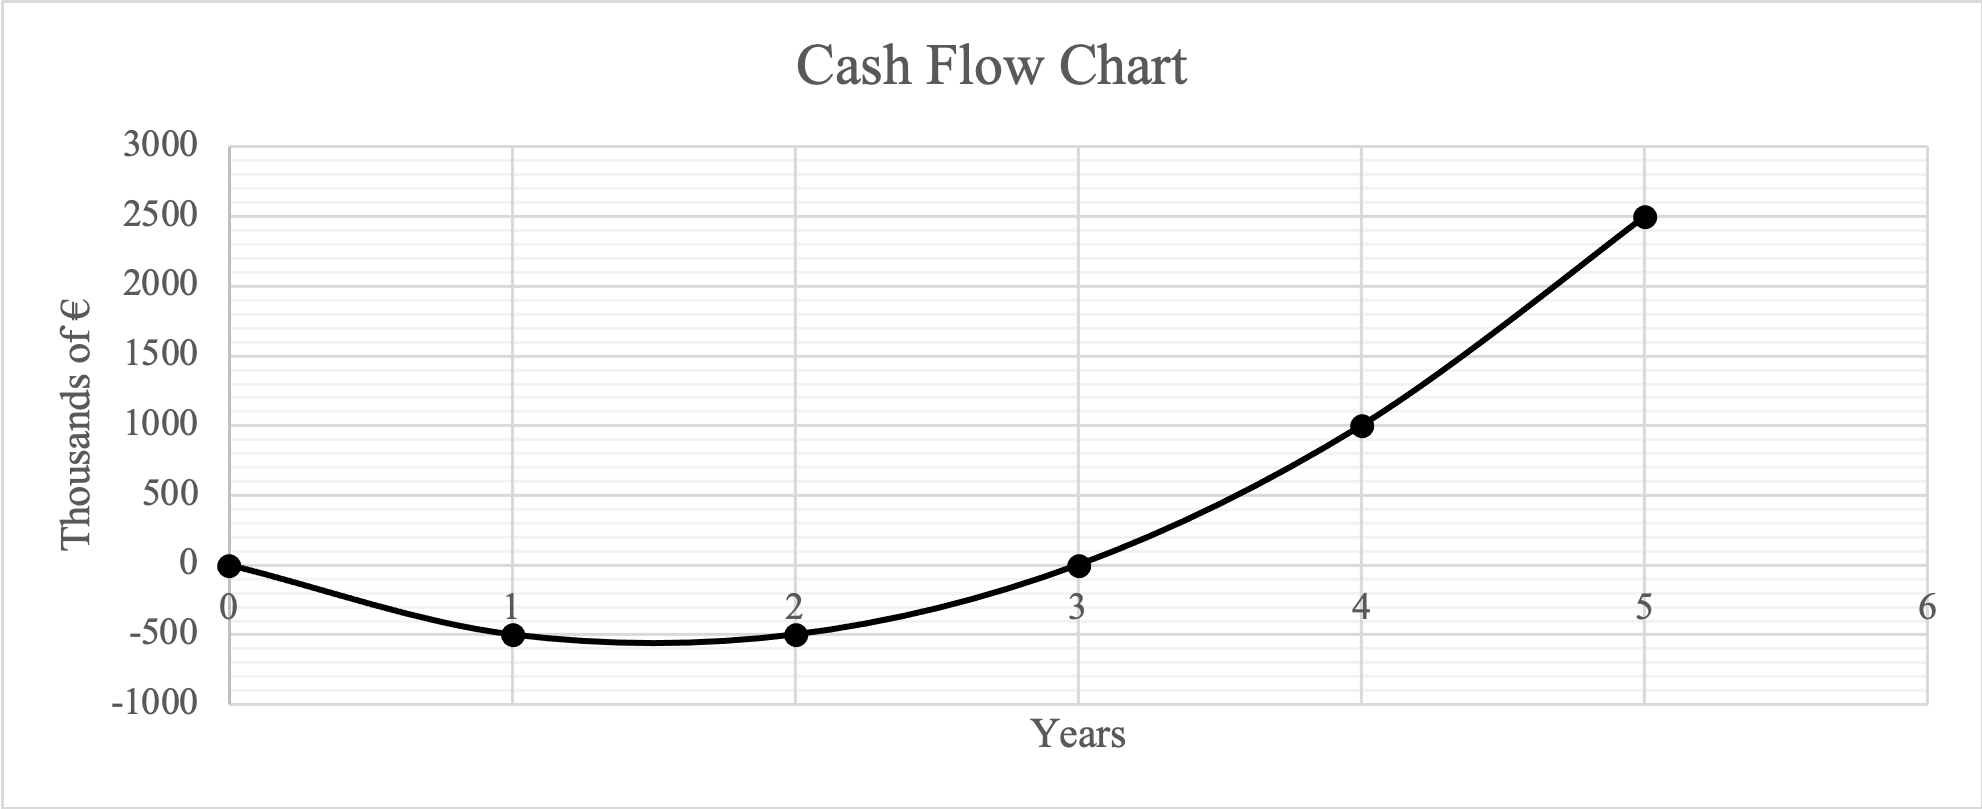
\includegraphics[width=0.8\textwidth]{images/Cash_Flow_Chart.png}
\caption{Estimated Cash Flow for the first 5 years}
\end{figure}
As can be seen in the chart above, the break-even point is expected to be reached in the third year, considering an upward trend of sales volumes. In addition, the variable costs will be mitigated by an accurate economy of scale strategy, with the support of our suppliers.

\begin{table}[H]
\centering
\caption{Financial projection for the first 5 years}
\begin{tabular}{GGccccm{0.1\textwidth}}
\toprule
&YEAR-1 & YEAR-2 &	YEAR-3 & YEAR-4 & YEAR-5\\
\hline
SALES VOLUMES &	0 & 21K & 35K & 60K & 100K\\
\hline
COSTS /€ & -500K & -800K &	-900K &	-1000K & -1100K\\
\hline
REVENUES /€ &	0 &	+800K &	+1400K &	+1900K &	+2800K\\
\hline
MARGIN /€ & -500K & -500K &	0 (BEP) &	1000K &	2500K\\
\bottomrule
\end{tabular}
\end{table}